\documentclass{standalone}
\usepackage{tikz}
\usetikzlibrary{patterns, positioning}


\begin{document}
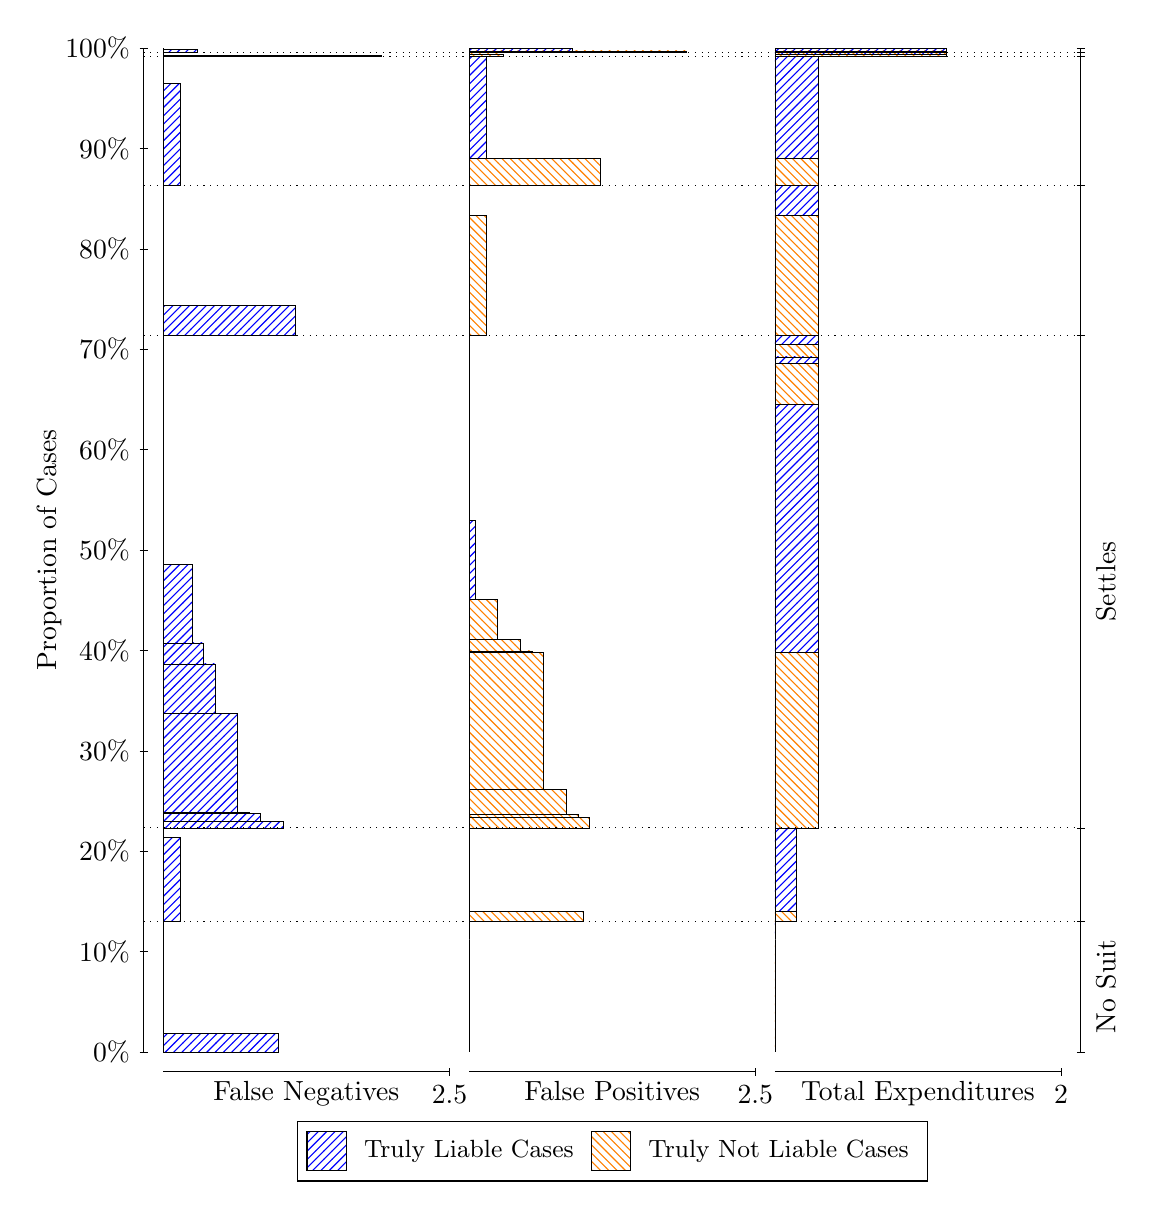
\begin{tikzpicture}
\draw[black, very thin] (1.5,1.75) -- (1.5,14.5);
\node[rotate=90, text=black, anchor=center] at (0.3, 8.125) {Proportion of Cases};
\draw[black, very thin] (1.45,1.75) -- (1.55,1.75);
\node[text=black, anchor=east] at (1.45, 1.75) {0\%};
\draw[black, very thin] (1.45,3.025) -- (1.55,3.025);
\node[text=black, anchor=east] at (1.45, 3.025) {10\%};
\draw[black, very thin] (1.45,4.3) -- (1.55,4.3);
\node[text=black, anchor=east] at (1.45, 4.3) {20\%};
\draw[black, very thin] (1.45,5.575) -- (1.55,5.575);
\node[text=black, anchor=east] at (1.45, 5.575) {30\%};
\draw[black, very thin] (1.45,6.85) -- (1.55,6.85);
\node[text=black, anchor=east] at (1.45, 6.85) {40\%};
\draw[black, very thin] (1.45,8.125) -- (1.55,8.125);
\node[text=black, anchor=east] at (1.45, 8.125) {50\%};
\draw[black, very thin] (1.45,9.4) -- (1.55,9.4);
\node[text=black, anchor=east] at (1.45, 9.4) {60\%};
\draw[black, very thin] (1.45,10.675) -- (1.55,10.675);
\node[text=black, anchor=east] at (1.45, 10.675) {70\%};
\draw[black, very thin] (1.45,11.95) -- (1.55,11.95);
\node[text=black, anchor=east] at (1.45, 11.95) {80\%};
\draw[black, very thin] (1.45,13.225) -- (1.55,13.225);
\node[text=black, anchor=east] at (1.45, 13.225) {90\%};
\draw[black, very thin] (1.45,14.5) -- (1.55,14.5);
\node[text=black, anchor=east] at (1.45, 14.5) {100\%};

\draw[black, very thin] (13.4,1.75) -- (13.4,14.5);
\draw[black, very thin] (13.35,1.75) -- (13.45,1.75);
\node[anchor=west] at (13.35, 1.75) {};
\draw[black, very thin] (13.35,3.4093) -- (13.45,3.4093);
\node[anchor=west] at (13.35, 3.4093) {};
\draw[black, very thin] (13.35,4.5954) -- (13.45,4.5954);
\node[anchor=west] at (13.35, 4.5954) {};
\draw[black, very thin] (13.35,10.852) -- (13.45,10.852);
\node[anchor=west] at (13.35, 10.852) {};
\draw[black, very thin] (13.35,12.753) -- (13.45,12.753);
\node[anchor=west] at (13.35, 12.753) {};
\draw[black, very thin] (13.35,14.389) -- (13.45,14.389);
\node[anchor=west] at (13.35, 14.389) {};
\draw[black, very thin] (13.35,14.445) -- (13.45,14.445);
\node[anchor=west] at (13.35, 14.445) {};
\draw[black, very thin] (13.35,14.5) -- (13.45,14.5);
\node[anchor=west] at (13.35, 14.5) {};

\draw[black, very thin, pattern color=blue, pattern=north east lines] (1.75,1.75) rectangle (3.2033,1.984);
\draw[black, very thin, pattern color=orange, pattern=north west lines] (1.75,1.984) rectangle (1.75,3.4093);
\draw[black, very thin, pattern color=blue, pattern=north east lines] (1.75,3.4093) rectangle (1.968,4.4706);
\draw[black, very thin, pattern color=orange, pattern=north west lines] (1.75,4.4706) rectangle (1.75,4.5954);
\draw[black, very thin, pattern color=blue, pattern=north east lines] (1.75,4.5954) rectangle (3.276,4.6827);
\draw[black, very thin, pattern color=blue, pattern=north east lines] (1.75,4.6827) rectangle (2.9853,4.7792);
\draw[black, very thin, pattern color=blue, pattern=north east lines] (1.75,4.7792) rectangle (2.84,4.7938);
\draw[black, very thin, pattern color=blue, pattern=north east lines] (1.75,4.7938) rectangle (2.6947,6.0475);
\draw[black, very thin, pattern color=blue, pattern=north east lines] (1.75,6.0475) rectangle (2.404,6.68);
\draw[black, very thin, pattern color=blue, pattern=north east lines] (1.75,6.68) rectangle (2.2587,6.9454);
\draw[black, very thin, pattern color=blue, pattern=north east lines] (1.75,6.9454) rectangle (2.1133,7.9472);
\draw[black, very thin, pattern color=orange, pattern=north west lines] (1.75,7.9472) rectangle (1.75,10.852);
\draw[black, very thin, pattern color=blue, pattern=north east lines] (1.75,10.852) rectangle (3.4213,11.23);
\draw[black, very thin, pattern color=orange, pattern=north west lines] (1.75,11.23) rectangle (1.75,12.753);
\draw[black, very thin, pattern color=blue, pattern=north east lines] (1.75,12.753) rectangle (1.968,14.048);
\draw[black, very thin, pattern color=orange, pattern=north west lines] (1.75,14.048) rectangle (1.75,14.389);
\draw[black, very thin, pattern color=blue, pattern=north east lines] (1.75,14.389) rectangle (4.5113,14.408);
\draw[black, very thin, pattern color=orange, pattern=north west lines] (1.75,14.408) rectangle (1.75,14.445);
\draw[black, very thin, pattern color=blue, pattern=north east lines] (1.75,14.445) rectangle (2.186,14.482);
\draw[black, very thin, pattern color=orange, pattern=north west lines] (1.75,14.482) rectangle (1.75,14.5);
\draw[black, very thin, pattern color=orange, pattern=north west lines] (5.6333,1.75) rectangle (5.6333,3.1753);
\draw[black, very thin, pattern color=blue, pattern=north east lines] (5.6333,3.1753) rectangle (5.6333,3.4093);
\draw[black, very thin, pattern color=orange, pattern=north west lines] (5.6333,3.4093) rectangle (7.0867,3.5341);
\draw[black, very thin, pattern color=blue, pattern=north east lines] (5.6333,3.5341) rectangle (5.6333,4.5954);
\draw[black, very thin, pattern color=orange, pattern=north west lines] (5.6333,4.5954) rectangle (7.1593,4.7315);
\draw[black, very thin, pattern color=orange, pattern=north west lines] (5.6333,4.7315) rectangle (7.014,4.7678);
\draw[black, very thin, pattern color=orange, pattern=north west lines] (5.6333,4.7678) rectangle (6.8687,5.0868);
\draw[black, very thin, pattern color=orange, pattern=north west lines] (5.6333,5.0868) rectangle (6.578,6.8253);
\draw[black, very thin, pattern color=orange, pattern=north west lines] (5.6333,6.8253) rectangle (6.4327,6.8451);
\draw[black, very thin, pattern color=orange, pattern=north west lines] (5.6333,6.8451) rectangle (6.2873,6.9885);
\draw[black, very thin, pattern color=orange, pattern=north west lines] (5.6333,6.9885) rectangle (5.9967,7.5007);
\draw[black, very thin, pattern color=blue, pattern=north east lines] (5.6333,7.5007) rectangle (5.706,8.5024);
\draw[black, very thin, pattern color=blue, pattern=north east lines] (5.6333,8.5024) rectangle (5.6333,10.852);
\draw[black, very thin, pattern color=orange, pattern=north west lines] (5.6333,10.852) rectangle (5.8513,12.375);
\draw[black, very thin, pattern color=blue, pattern=north east lines] (5.6333,12.375) rectangle (5.6333,12.753);
\draw[black, very thin, pattern color=orange, pattern=north west lines] (5.6333,12.753) rectangle (7.3047,13.094);
\draw[black, very thin, pattern color=blue, pattern=north east lines] (5.6333,13.094) rectangle (5.8513,14.389);
\draw[black, very thin, pattern color=orange, pattern=north west lines] (5.6333,14.389) rectangle (6.0693,14.426);
\draw[black, very thin, pattern color=blue, pattern=north east lines] (5.6333,14.426) rectangle (5.6333,14.445);
\draw[black, very thin, pattern color=orange, pattern=north west lines] (5.6333,14.445) rectangle (8.3947,14.463);
\draw[black, very thin, pattern color=blue, pattern=north east lines] (5.6333,14.463) rectangle (6.9413,14.5);
\draw[black, very thin, pattern color=orange, pattern=north west lines] (9.5167,1.75) rectangle (9.5167,3.1753);
\draw[black, very thin, pattern color=blue, pattern=north east lines] (9.5167,3.1753) rectangle (9.5167,3.4093);
\draw[black, very thin, pattern color=orange, pattern=north west lines] (9.5167,3.4093) rectangle (9.7892,3.5341);
\draw[black, very thin, pattern color=blue, pattern=north east lines] (9.5167,3.5341) rectangle (9.7892,4.5954);
\draw[black, very thin, pattern color=orange, pattern=north west lines] (9.5167,4.5954) rectangle (10.062,6.8253);
\draw[black, very thin, pattern color=blue, pattern=north east lines] (9.5167,6.8253) rectangle (10.062,9.9786);
\draw[black, very thin, pattern color=orange, pattern=north west lines] (9.5167,9.9786) rectangle (10.062,10.491);
\draw[black, very thin, pattern color=blue, pattern=north east lines] (9.5167,10.491) rectangle (10.062,10.578);
\draw[black, very thin, pattern color=orange, pattern=north west lines] (9.5167,10.578) rectangle (10.062,10.741);
\draw[black, very thin, pattern color=blue, pattern=north east lines] (9.5167,10.741) rectangle (10.062,10.852);
\draw[black, very thin, pattern color=orange, pattern=north west lines] (9.5167,10.852) rectangle (10.062,12.375);
\draw[black, very thin, pattern color=blue, pattern=north east lines] (9.5167,12.375) rectangle (10.062,12.753);
\draw[black, very thin, pattern color=orange, pattern=north west lines] (9.5167,12.753) rectangle (10.062,13.094);
\draw[black, very thin, pattern color=blue, pattern=north east lines] (9.5167,13.094) rectangle (10.062,14.389);
\draw[black, very thin, pattern color=orange, pattern=north west lines] (9.5167,14.389) rectangle (11.697,14.426);
\draw[black, very thin, pattern color=blue, pattern=north east lines] (9.5167,14.426) rectangle (11.697,14.445);
\draw[black, very thin, pattern color=orange, pattern=north west lines] (9.5167,14.445) rectangle (11.697,14.463);
\draw[black, very thin, pattern color=blue, pattern=north east lines] (9.5167,14.463) rectangle (11.697,14.5);
\draw[black, dotted] (1.5,3.4093) -- (13.4,3.4093);
\draw[black, dotted] (1.5,4.5954) -- (13.4,4.5954);
\draw[black, dotted] (1.5,10.852) -- (13.4,10.852);
\draw[black, dotted] (1.5,12.753) -- (13.4,12.753);
\draw[black, dotted] (1.5,14.389) -- (13.4,14.389);
\draw[black, dotted] (1.5,14.445) -- (13.4,14.445);
\draw[black, very thin] (1.75,1.5) -- (5.3833,1.5);
\node[text=black, anchor=north] at (3.5667, 1.5) {False Negatives};
\draw[black, very thin] (5.3833,1.45) -- (5.3833,1.55);
\node[text=black, anchor=north] at (5.3833, 1.45) {2.5};

\draw[black, very thin] (5.6333,1.5) -- (9.2667,1.5);
\node[text=black, anchor=north] at (7.45, 1.5) {False Positives};
\draw[black, very thin] (9.2667,1.45) -- (9.2667,1.55);
\node[text=black, anchor=north] at (9.2667, 1.45) {2.5};

\draw[black, very thin] (9.5167,1.5) -- (13.15,1.5);
\node[text=black, anchor=north] at (11.333, 1.5) {Total Expenditures};
\draw[black, very thin] (13.15,1.45) -- (13.15,1.55);
\node[text=black, anchor=north] at (13.15, 1.45) {2};

\node[text=black, centered, rotate=90] at (13.72, 2.5796) {No Suit};

\node[text=black, centered, rotate=90] at (13.72, 7.7239) {Settles};





\draw (7.449999999999999,1.5) node[draw=none] (baseCoordinate) {};
\begin{scope}[align=center]
        \matrix[scale=0.5, draw=black, below=0.5cm of baseCoordinate, nodes={draw}, column sep=0.1cm]{
            \node[rectangle, draw, minimum width=0.5cm, minimum height=0.5cm, pattern color=blue, pattern=north east lines] {}; &
            \node[draw=none, font=\small, text=black] (B) {Truly Liable Cases}; &
            \node[rectangle, draw, minimum width=0.5cm, minimum height=0.5cm, pattern color=orange, pattern=north west lines] {}; &
            \node[draw=none, font=\small, text=black] (B) {Truly Not Liable Cases}; \\
            };
\end{scope}

\end{tikzpicture}
\end{document}